%-shell-escape, якщо використовуєте minted
\documentclass[a4paper, 12pt, oneside]{extarticle}
\input{$HOME/Templates/lpnu_doc_templates/settings/preamble.tex}
% якщо домахуються за Times New Roman, то
% використовуєте xelatex і цей файл:
\input{$HOME/Templates/lpnu_doc_templates/settings/font_styles.tex}

\newcommand\Variant{12}
\newcommand\Date{12.05.\the\year}
\newcommand\Discipline{Комп'ютерна схемотехніка та архітектура комп'ютерних систем}
\newcommand\Instructor{Чкалов О. В.}

\newcommand\Type{\Lab}
\newcommand\Number{2}
\newcommand\Topic{Дослідження логічних елементів}
\graphicspath{{images/}}

\begin{document}
\Margins

\Margins
%\begin{wrapfigure}[3]{l}{.27\textwidth}
%\includegraphics[width=.28\textwidth]{$UNI/.templates/lpnu_logo.png}
%\end{wrapfigure}

%\noindent\textbf{Прізвище:} \Lname \\
%\noindent\textbf{Ім'я:} \Fname \\
%\noindent\textbf{Група:} \Group \\
%\noindent\textbf{Варіант:} \Variant \\
%\noindent\textbf{Дата захисту:} \Date \\
%\\
%\noindent\textbf{Кафедра:} \Department \\
%\noindent\textbf{Дисципліна:} \Discipline \\
%\noindent\textbf{Перевірив:} \Instructor \\

%%\medskip\bigskip

%\begin{center}
%	\textbf{ЗВІТ}		\\
%	до \Type~\No\Number	\\
%	на тему ``\Topic''	\\
%\end{center}

% \begin{table}
%   \begin{tabularx}{\textwidth}{|c|X|X|}
%     \hline
%     % Image & Content & Additional Info \\
%     % \hline
% 	  \multirow{3}{*}{\includegraphics[width=4cm]{$UNI/.templates/lpnu_logo.png}}
% 	  & \textbf{ЗВО:}
% 	  Національний університет ``Львівська Політехніка''.
% 	  & \textbf{Тема:}
% 	  \Topic
% 	  \\
% 	  & \textbf{Навчальний рік:}
% 	  2023/2024
% 	  & \textbf{Інститут}
% 	  комп'ютерних наук та інформаційних технологій
% 	  \\
% 	  & \textbf{Семестр:}
% 	  осінній
% 	  & \textbf{Група:}
% 	  \Group
% 	  \\
% 	  & \textbf{Навчальна дисципліна:}
% 	  \Discipline
% 	  & \textbf{Студент:}
% 	  Мілюхін Олександр
% 	  \\
% 	  & \textbf{Кафедра}
% 	  систем автоматизованого проектування
% 	  &
% 	  \\
% 	  & \textbf{Викладач:}
% 	  Чумакевич В. В.
% 	  &
% 	  \\
%     \hline
%   \end{tabularx}
% \end{table}

\setlength{\textfloatsep}{-16pt}
% \setlength{\intextsep}{0pt}

\begin{table}
	\begin{tabular}{|l|l|p{6cm}|}
    \hline
    % Image & Content & Additional Info \\
    % \hline
	  \makecell[l]{
	  \includegraphics[width=3.37cm]{$UNI/.templates/lpnu_logo.png}
  }
	  & \makecell[l]{
	  \textbf{ЗВО:}
	  Національний університет \\ ``Львівська Політехніка''.
	  \\
	  \textbf{Навчальний рік:}
	  2023/2024
	  \\
	  \textbf{Семестр:}
	  осінній
	  \\
	  \textbf{Навчальна дисципліна:} \\
	  \Discipline
	  \\
	  \textbf{Кафедра}
	  систем автоматизованого \\ проектування
	  \\
	  \textbf{Викладач:}
	  Чумакевич В. В.
}
	  & \makecell [l] {
	  \textbf{Тема:}
	  \Topic
	  \\
          \textbf{Інститут}
	  комп'ютерних наук та \\ інформаційних технологій
	  \\
	  \textbf{Група:}
	  \Group
	  \\
	  \textbf{Студент:}
	  Мілюхін Олександр
  }
  \\
    \hline
  \end{tabular}
\end{table}
\section{Мета роботи}

% \begin{table}
%   \begin{tabularx}{\textwidth}{|p{6cm}|c|c|}
% 	  \hline
%     \multirow{3}{*}{\includegraphics[width=6cm]{$UNI/.templates/lpnu_logo.png}}
% 	  & ЗВО: Національний університет ``Львівська Політехніка''
% 	  & Additional Info 1 \\
%     & Content 2 & Additional Info 2 \\
%     & Content 3 & Additional Info 3 \\
% 	  \hline
%   \end{tabularx}
% \end{table}

% \begin{table}
%   \begin{tabular}{|c|c|c|}
%     \hline
%     \multirow{3}{*}{\includegraphics[width=3cm]{$UNI/.templates/lpnu_logo.png}} & \makecell{Content 1 \\ Content 2 \\ Content 3} & \makecell{Additional Info 1 \\ Additional Info 2 \\ Additional Info 3} \\
%     \hline
%   \end{tabular}
% \end{table}


дослідити роботу та принципи побудови логічних елементів
на резистивно-транзисторній логіці та МОН-транзисторах.

\section*{Індивідуальне завдання}

\subsection*{Завдання 1}

\begin{tabular}{c||c}
	12 & І-НЕ, НЕ, ЧИ-НЕ (РТЛ), ЧИ, І (МОН)
\end{tabular}

\subsection*{Завдання 2}

Побудувати чотири схеми в програмі NI Mutisim на логічних елементах та
використовуючи мікросхеми цих логічних елементів.
\paragraph{1} побудувати задану схему на логічних елементах і на
мікросхемах КМОН 4000 – серії, отримати логічну функцію по схемі та її
таблицю істинності використовуючи логічний перетворювач (Logic converter).
\paragraph{2} побудувати схему на логічних елементах і на мікросхемах
КМОН 4000 – серії по заданій логічній функції, отримати за логічною схемою
таблицю істинності досліджуваної логічної функції використовуючи логічний
перетворювач (Logic converter).

\begin{figure}[h]
	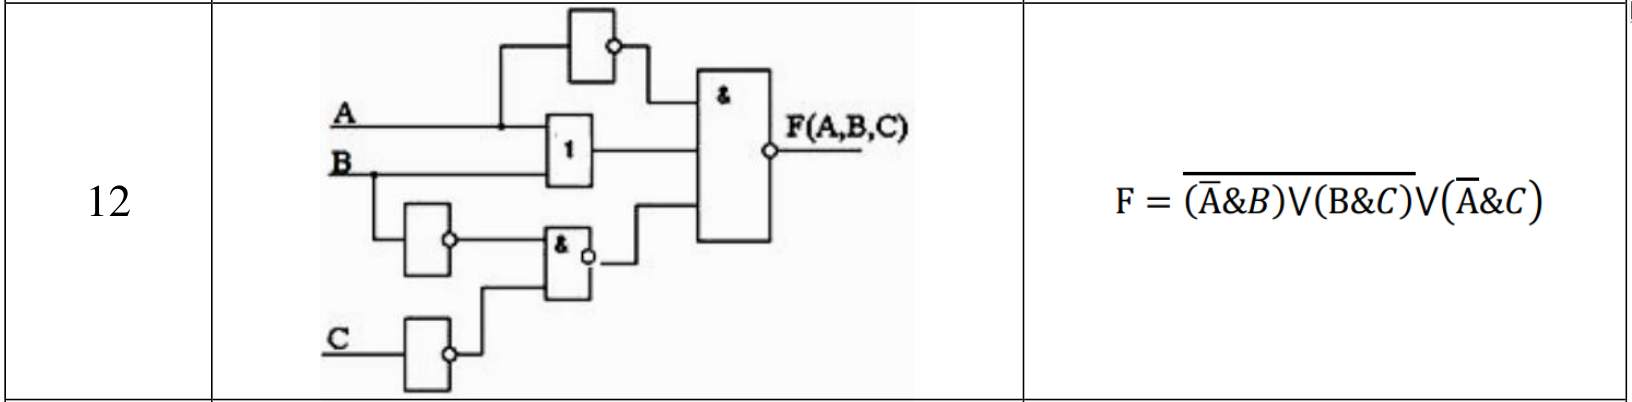
\includegraphics[width=\textwidth]{task_2}
	% \caption{І-НЕ}
\end{figure}

\section*{Етапи розв'язку}

\subsection*{Завдання 1}

\begin{figure}[h]
	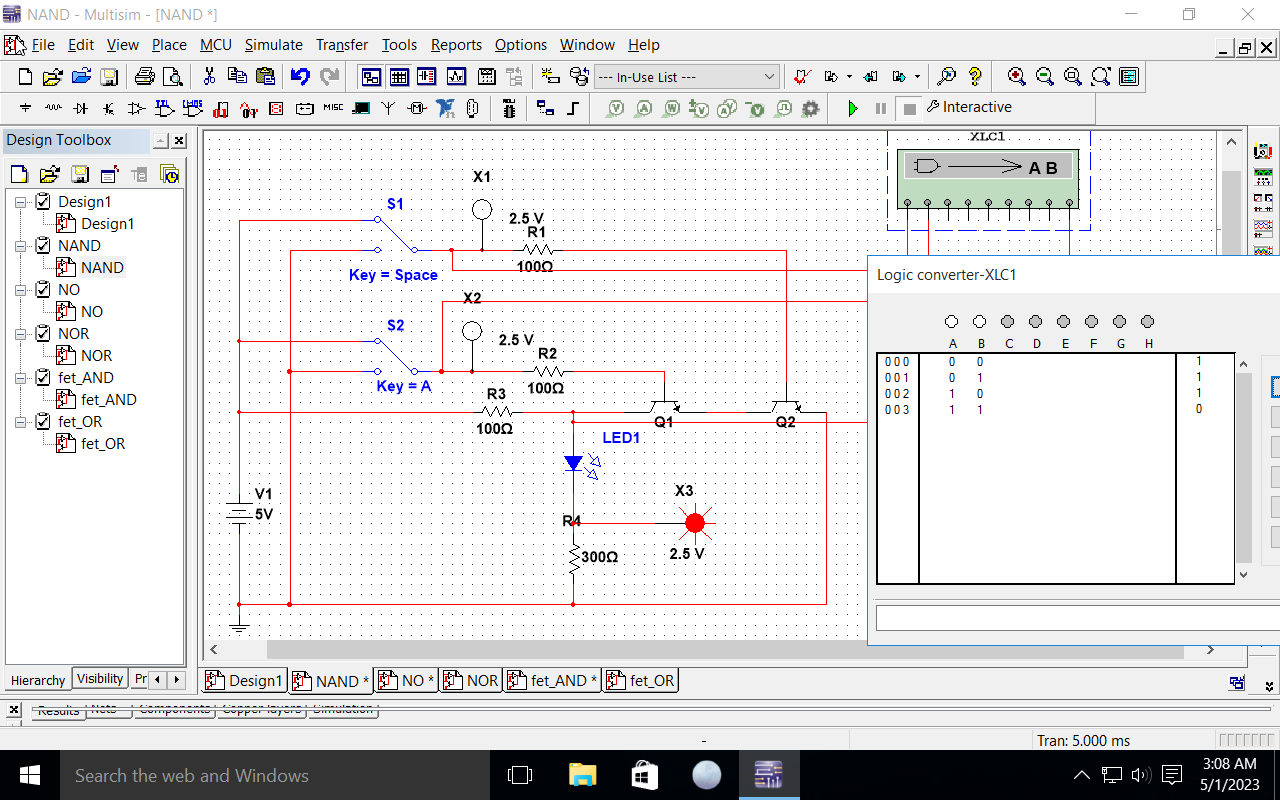
\includegraphics[width=\textwidth]{NAND}
	\caption{І-НЕ}
\end{figure}
\begin{figure}[h]
	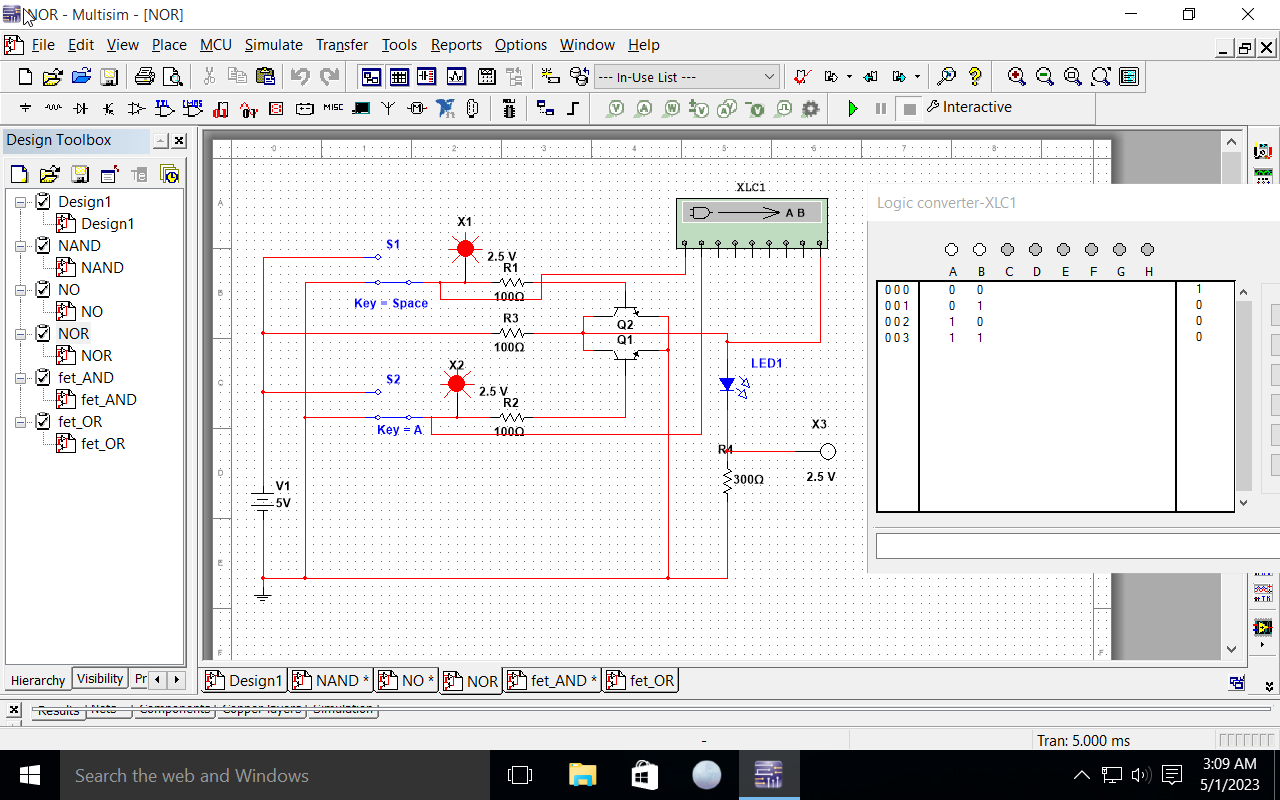
\includegraphics[width=\textwidth]{NOR}
	\caption{ЧИ-НЕ}
\end{figure}
\begin{figure}[h]
	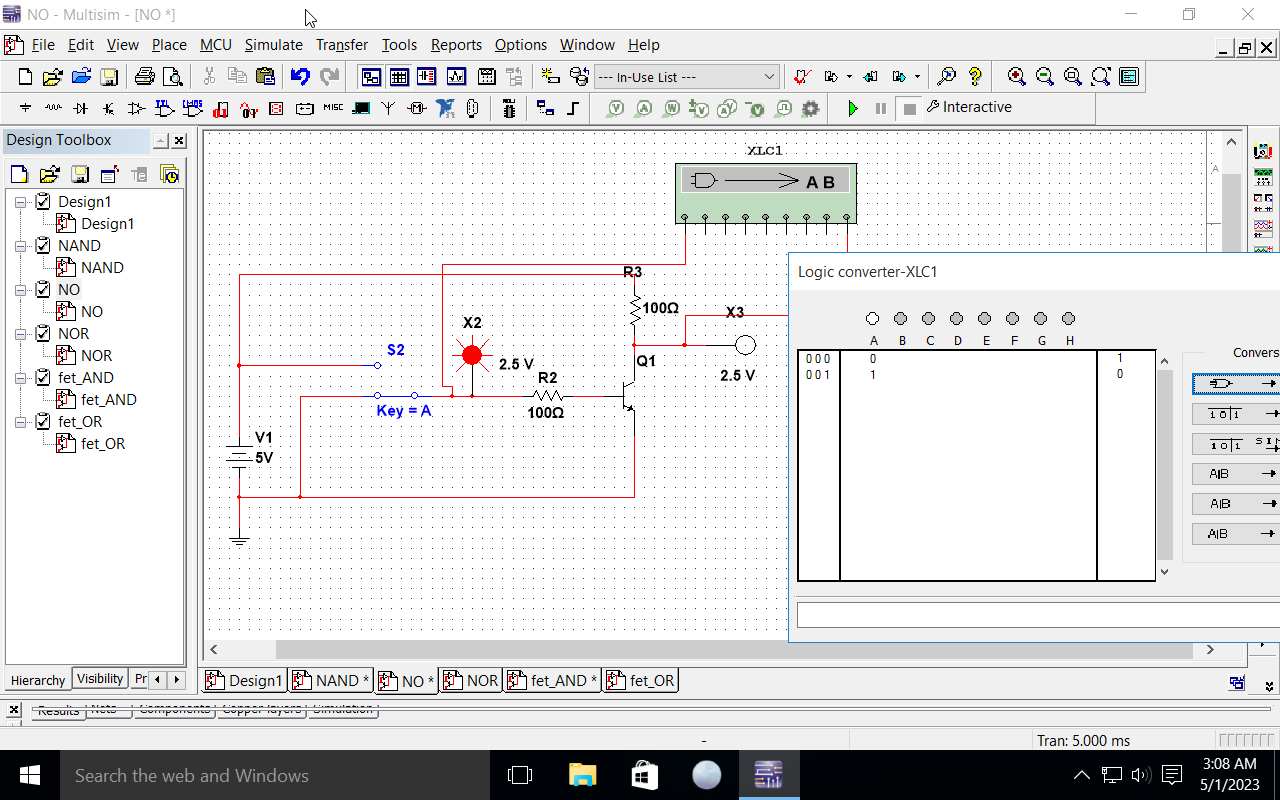
\includegraphics[width=\textwidth]{NO}
	\caption{НЕ}
\end{figure}
\begin{figure}[h]
	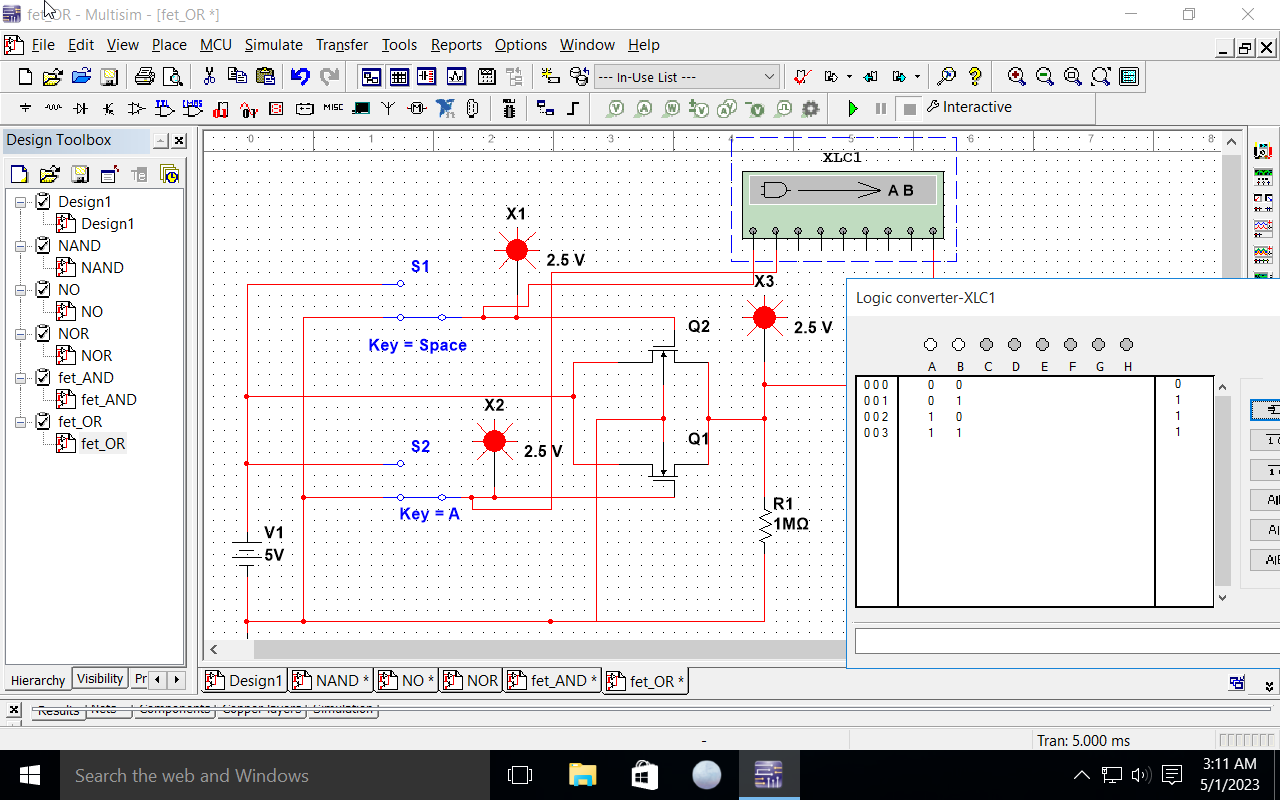
\includegraphics[width=\textwidth]{fet_OR}
	\caption{АБО (МОН)}
\end{figure}
\begin{figure}[ht]
	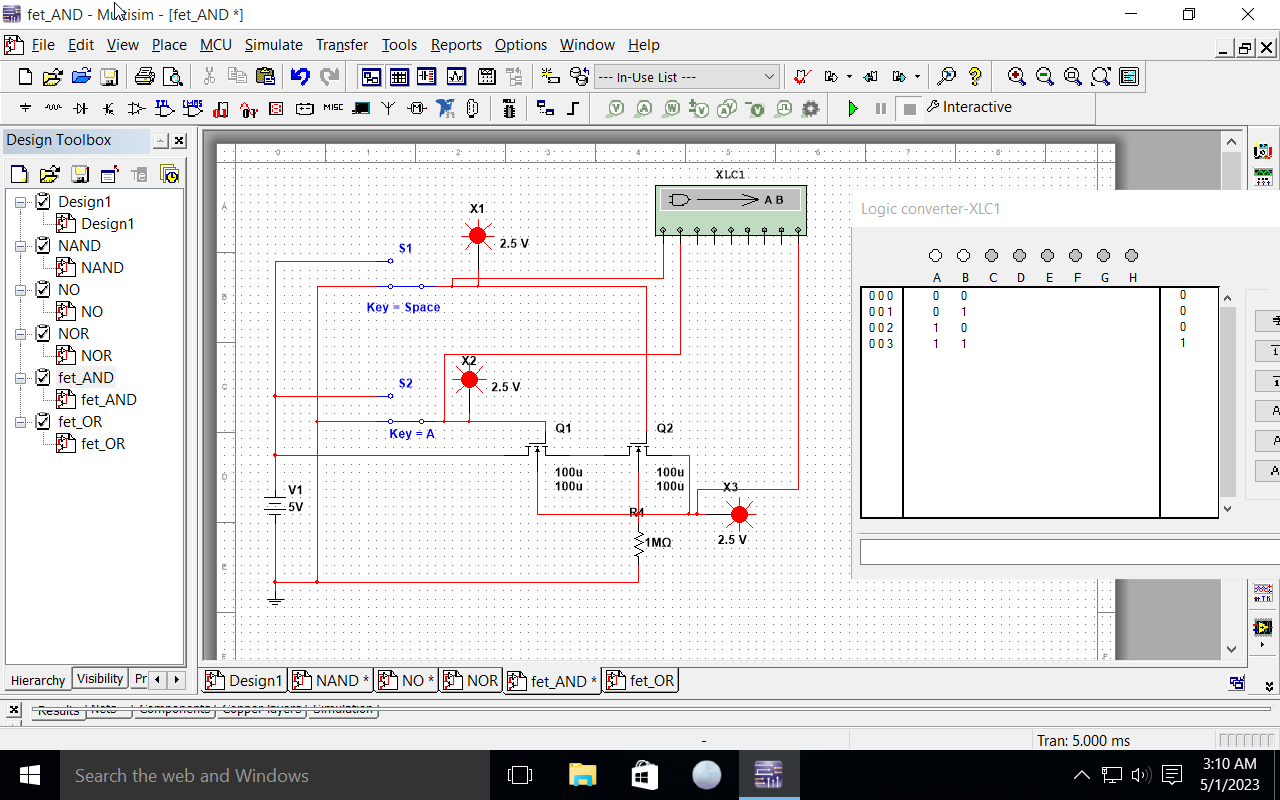
\includegraphics[width=\textwidth]{fet_AND}
	\caption{І (МОН)}
\end{figure}

\clearpage

\subsection*{Завдання 2}

\begin{figure}[h]
	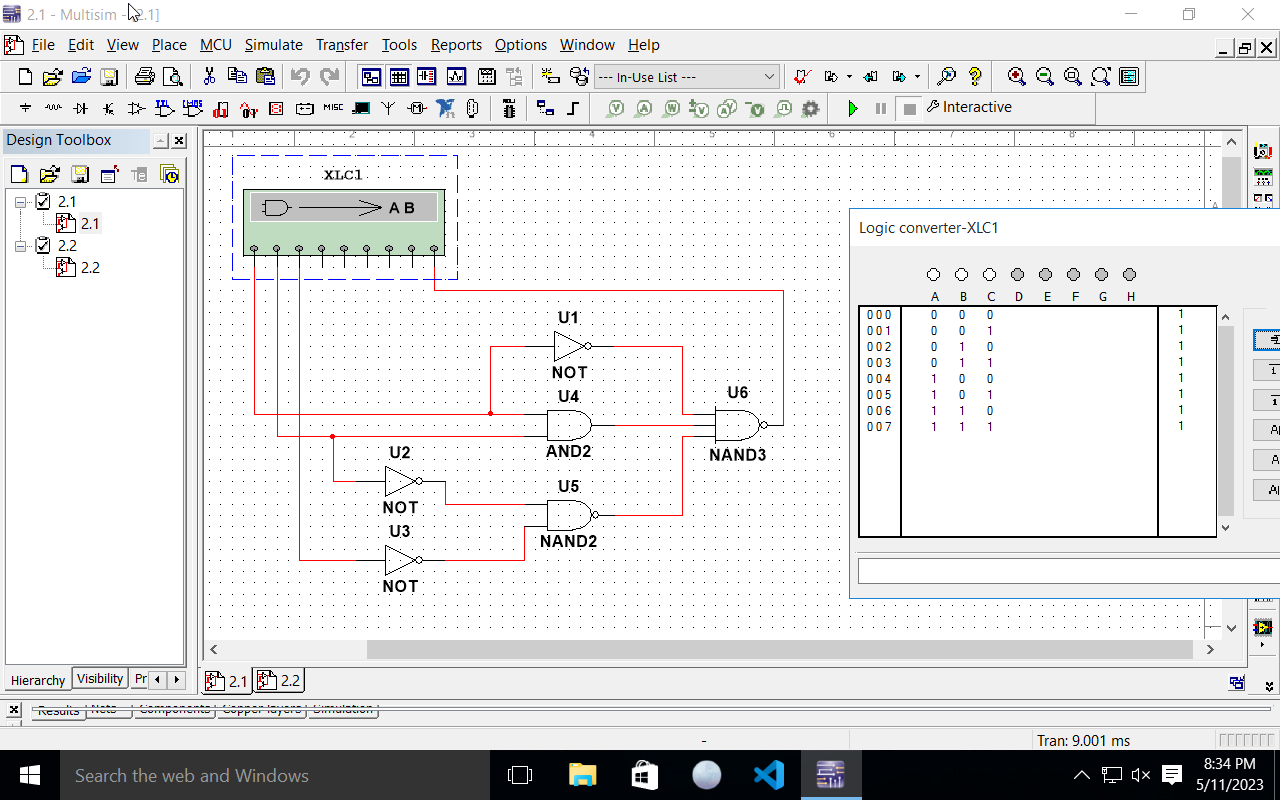
\includegraphics[width=\textwidth]{2.1}
	\caption{1 частина завдання}
\end{figure}
\begin{figure}[h]
	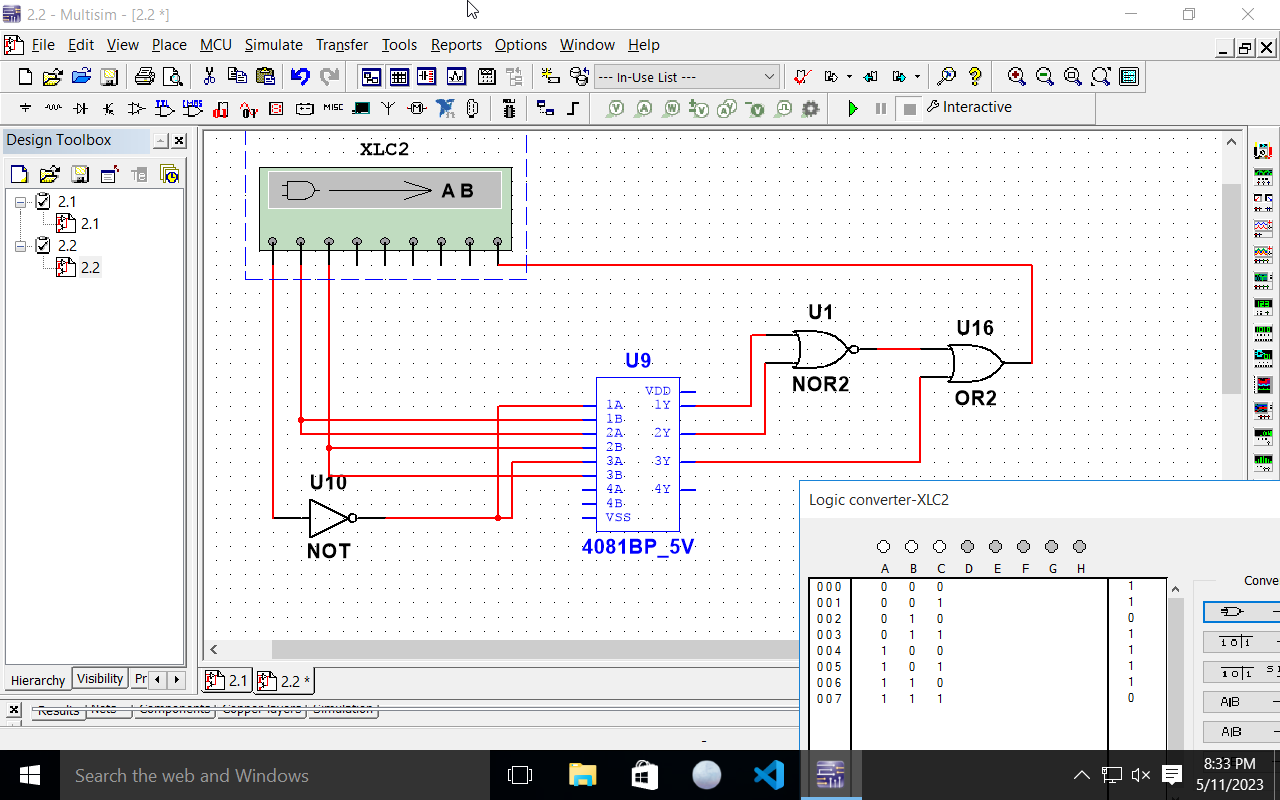
\includegraphics[width=\textwidth]{2.2}
	\caption{2 частина завдання}
\end{figure}

\clearpage

\section*{Висновок}

Дослідив роботу та принципи побудови логічних елементів на резистивно-транзисторній логіці та МОН-транзисторах,
побудував схеми логічних функцій.

\section*{Відповіді на контрольні запитання}
\begin{itemize}
	\question Які існують логічні операції?
		\answer Кон'юнкція, диз'юнкція, імплікація, рівносильність(еквівалентність), заперечення та інші.

	\question Що називається логічним елементом?
	\answer Логічний елемент - це електронний пристрій або компонент, який виконує логічні операції над сигналами логічних змінних

	\question Які логічні елементи реалізують логічні операції?
		\answer Заперечення реалізує інвертор (НЕ), диз'юнкцію --- елемент ЧИ, кон'юнкцію --- І, заперечення диз'юнкції --- НЕ ЧИ, зап. кон'юнкції --- НЕ І.

	\question Вказати область застосування логічних елементів.
	\answer Побудова логічних схем, мікропроцесорів, логічних вентилів.

	\question Якими методами описують логічні операції?
	\answer Логічні операції описують за допомогою:
		\begin{itemize}
	\item таблиць істинності
	\item булевих функцій
	\item графічного методу
	\item алгебраїчного методу
		\end{itemize}
\end{itemize}

\end{document}
